\documentclass[11pt,oneside,openany]{book}

\usepackage[
  paperwidth=6in,
  paperheight=9in,
  inner=0.75in,
  outer=0.5in,
  top=0.5in,
  bottom=0.5in,
  headheight=14pt,
  headsep=12pt,
  footskip=20pt
]{geometry}

\usepackage{amsmath,amssymb,amsthm,mathtools}
\usepackage{booktabs,longtable,array,multirow,tabularx}
\usepackage{enumitem}
\usepackage[dvipsnames,svgnames,x11names]{xcolor}
\usepackage{tikz}
\usetikzlibrary{shapes.geometric,arrows.meta,positioning}
\usepackage{float}
\usepackage{caption}
\usepackage{microtype}
\usepackage{setspace}
\usepackage{titlesec}
\usepackage{fancyhdr}
\usepackage[most]{tcolorbox}
\usepackage{qrcode}
\usepackage{adjustbox}
\usepackage{hyperref}
\usepackage{bookmark}

\onehalfspacing

\setlength{\parindent}{0pt}
\setlength{\parskip}{6pt plus 2pt minus 1pt}

\newcommand{\BookTitle}{AP\textsuperscript{\textregistered} Statistics Formula \& Inference Decision Guide}
\newcommand{\BookSubtitle}{The High-Yield Score-5 Cram Companion: Rapid Formula Breakdowns, Inference Decision Trees, and Fill-in-the-Blank FRQ Sentence Frames}
\newcommand{\BookSeries}{AP\textsuperscript{\textregistered} Statistics Score-5 Blueprint Series --- Volume 1}
\newcommand{\BookAuthor}{PR}
\newcommand{\Edition}{2027 Exam Edition}

% Header & Footer (Strict KDP Safe Boundary >= 0.25in from trim)
\pagestyle{fancy}
\fancyhf{}
\fancyhead[LE]{\small\itshape \BookTitle}
\fancyhead[RO]{\small\itshape \leftmark}
\fancyfoot[C]{\small\thepage}
\renewcommand{\headrulewidth}{0.4pt}
\renewcommand{\footrulewidth}{0pt}

% Section styling
\titleformat{\chapter}[display]
  {\normalfont\Large\bfseries\color{MidnightBlue}}{\chaptertitlename\ \thechapter}{10pt}{\LARGE\bfseries}
\titleformat{\section}
  {\normalfont\large\bfseries\color{MidnightBlue}}{\thesection}{1em}{}
\titleformat{\subsection}
  {\normalfont\normalsize\bfseries\color{DarkSlateGray}}{\thesubsection}{1em}{}

% Custom TColorBoxes for Professional KDP Interior (Strict No-Bleed / Breakable Enabled)
\newtcolorbox{formulabox}[1][]{
  enhanced,
  breakable,
  colback=NavyBlue!5!white,
  colframe=NavyBlue!80!black,
  fonttitle=\bfseries\color{white},
  title={#1},
  arc=2.5mm,
  boxrule=1pt,
  left=8pt,
  right=8pt,
  top=6pt,
  bottom=6pt,
  before skip=8pt,
  after skip=8pt
}

\newtcolorbox{trapbox}[1][]{
  enhanced,
  breakable,
  colback=Red!5!white,
  colframe=Red!80!black,
  fonttitle=\bfseries\color{white},
  title={#1},
  arc=2.5mm,
  boxrule=1pt,
  left=8pt,
  right=8pt,
  top=6pt,
  bottom=6pt,
  before skip=8pt,
  after skip=8pt
}

\newtcolorbox{templatebox}[1][]{
  enhanced,
  breakable,
  colback=ForestGreen!5!white,
  colframe=ForestGreen!85!black,
  fonttitle=\bfseries\color{white},
  title={#1},
  arc=2.5mm,
  boxrule=1pt,
  left=8pt,
  right=8pt,
  top=6pt,
  bottom=6pt,
  before skip=8pt,
  after skip=8pt
}

\newtcolorbox{tipbox}[1][]{
  enhanced,
  breakable,
  colback=Amber!8!white,
  colframe=DarkOrange!90!black,
  fonttitle=\bfseries\color{white},
  title={#1},
  arc=2.5mm,
  boxrule=1pt,
  left=8pt,
  right=8pt,
  top=6pt,
  bottom=6pt,
  before skip=8pt,
  after skip=8pt
}

\newtcolorbox{calloutbox}[1][]{
  enhanced,
  breakable,
  colback=SlateGray!8!white,
  colframe=SlateGray!90!black,
  fonttitle=\bfseries\color{white},
  title={#1},
  arc=2.5mm,
  boxrule=1pt,
  left=8pt,
  right=8pt,
  top=6pt,
  bottom=6pt,
  before skip=8pt,
  after skip=8pt
}

\hypersetup{
  colorlinks=true,
  linkcolor=NavyBlue,
  citecolor=NavyBlue,
  urlcolor=NavyBlue
}

\begin{document}

\frontmatter

% TITLE PAGE
\begin{titlepage}
\centering
\vspace*{0.8in}

{\Large\scshape \BookSeries}\par
\vspace{1.2cm}

{\Huge\bfseries\color{MidnightBlue} \BookTitle}\par
\vspace{0.6cm}
{\Large\itshape \BookSubtitle}\par

\vspace{2cm}

\rule{0.6\linewidth}{1.2pt}\par
\vspace{1.5cm}

{\Large\bfseries \BookAuthor}\par
\vspace{0.4cm}
{\large \Edition}\par

\vfill

{\small Published for Independent Amazon KDP Distribution}\par
\vspace*{0.5in}
\end{titlepage}

% COPYRIGHT PAGE
\newpage
\thispagestyle{empty}
\vspace*{2.5in}

\noindent \copyright\ 2027 \BookAuthor. All rights reserved.\\
No part of this publication may be reproduced, distributed, or transmitted in any form or by any means, including photocopying, recording, or other electronic or mechanical methods, without the prior written permission of the author and publisher, except in the case of brief quotations embodied in critical reviews and certain other noncommercial uses permitted by copyright law.

\vspace{0.3in}

\noindent \textbf{\textregistered\ Trademark Notice \& Nominative Fair Use Disclaimer:}\\
\small{AP\textregistered\ and Advanced Placement\textregistered\ are trademarks registered by the College Board, which was not involved in the production of, and does not endorse, this product. TI-84\textregistered\ is a registered trademark of Texas Instruments. All trademarks, service marks, and trade names referred to in this book are the property of their respective owners and are used herein for nominative, educational, and descriptive purposes only under Fair Use rules.}

\vspace{0.2in}

\noindent \textbf{Free Companion Online Portal \& Resources:}\\
Access downloadable PDF cheat sheets, interactive diagnostic drills, and live formula lookups:

\begin{center}
    \vspace{0.1in}
    \adjustbox{max width=\linewidth}{%
      \qrcode[height=1.2in]{https://narayanakdp.github.io/ap-stats-score5-blueprint/}%
    }
    
    \vspace{0.08in}
    {\footnotesize\textbf{\textsf{Scan on Mobile to Access Interactive Web Companion}}}\\
    {\scriptsize\texttt{https://narayanakdp.github.io/ap-stats-score5-blueprint/}}
\end{center}

\vspace{0.15in}
\noindent Published Independently via Amazon KDP\\
First Edition: 2027\\
ISBN / ASIN: Assigned by Amazon KDP

% HOW TO USE
\chapter*{How to Use This Companion to Score a 5}
\addcontentsline{toc}{chapter}{How to Use This Companion to Score a 5}

Welcome to the \textbf{AP Statistics Formula \& Inference Decision Guide}! This book was engineered specifically to solve the two biggest complaints students have with standard AP prep books:
\begin{enumerate}
    \item \textbf{Textbook Bloat:} Standard books are 600+ pages of dense theory that take weeks to read.
    \item \textbf{The FRQ Point Leak:} Students lose partial credit on Free-Response Questions not because their math is wrong, but because their verbal phrasing fails to satisfy strict AP rubric wording.
\end{enumerate}

\section*{The 3-Step Score-5 System}

\begin{enumerate}[label=\textbf{Step \arabic*:}]
    \item \textbf{Master the Formulas \& Parameters (Chapters 1--9):} For every formula on the official College Board reference sheet, review the plain-English parameter translation, when to use it, and what conditions are required.
    \item \textbf{Navigate the Master Inference Flowchart (Chapter 10):} Before starting any hypothesis test or confidence interval problem, follow the decision tree to ensure you select the correct procedure without second-guessing.
    \item \textbf{Eliminate Grader Traps \& Memorize Sentence Frames (Chapters 11--12):} Read through the Top 25 Exam Traps and adopt the exact fill-in-the-blank sentence frames for $p$-values, confidence levels, slope, and $r^2$ so that graders award you full points.
\end{enumerate}

\begin{tipbox}[Pro Tip for the Final 14 Days Before Exam Day]
Don't re-read entire textbooks. Spend 20 minutes each morning reviewing one unit's cheat sheet box and 10 minutes writing out the conditions checklist from memory.
\end{tipbox}

\tableofcontents

\mainmatter

% UNIT 1
\chapter{Unit 1: Exploring One-Variable Data}
\section{Essential Concepts \& Cheat Sheet}
When describing any quantitative single-variable distribution on the AP Exam, you \textbf{must} address four key characteristics: \textbf{SOCS} (Shape, Outliers, Center, Spread) always written \textbf{in context} of the problem.

\begin{formulabox}[Core Formulas: One-Variable Statistics]
\textbf{1. Mean ($\bar{x}$):} $\bar{x} = \frac{\sum x_i}{n} = \frac{1}{n} \sum x_i$

\textbf{2. Sample Standard Deviation ($s_x$):} $s_x = \sqrt{\frac{1}{n-1}\sum (x_i - \bar{x})^2}$

\textbf{3. Standardized Score ($z$-score):} $z = \frac{x - \mu}{\sigma} \quad \text{or} \quad z = \frac{x - \bar{x}}{s_x}$
\end{formulabox}

\section{Outlier Identification Rules}
\begin{itemize}
    \item \textbf{1.5 $\times$ IQR Rule:} $\text{IQR} = Q_3 - Q_1$. Outliers are values $< Q_1 - 1.5(\text{IQR})$ or $> Q_3 + 1.5(\text{IQR})$.
    \item \textbf{2-SD Rule (Normal data):} Outliers are values outside $\mu \pm 2\sigma$.
\end{itemize}

\section{Resistant vs. Non-Resistant Summary Statistics}
\begin{table}[H]
\centering
\small
\begin{tabularx}{\linewidth}{@{}l X X@{}}
\toprule
\textbf{Measure} & \textbf{Resistant to Outliers / Skew?} & \textbf{When to Use on Exam} \\
\midrule
\textbf{Median} & \textbf{Yes} (Unaffected by extremes) & Skewed distributions \\
\textbf{IQR} & \textbf{Yes} (Middle 50\% only) & Skewed distributions \\
\textbf{Mean} & \textbf{No} (Pulled toward tail/outliers) & Symmetric, unimodal distributions \\
\textbf{Standard Deviation} & \textbf{No} (Squared deviations inflate) & Symmetric, unimodal distributions \\
\bottomrule
\end{tabularx}
\end{table}

\begin{trapbox}[AP Exam Trap Alert: Comparing Distributions]
When comparing two distributions on an FRQ:
\begin{enumerate}
    \item You \textbf{must} use comparative words (e.g., \emph{"Distribution A has a greater median than Distribution B"}).
    \item You \textbf{must} include context (e.g., grams of sugar, test scores, heights).
\end{enumerate}
\end{trapbox}

% UNIT 2
\chapter{Unit 2: Exploring Two-Variable Data}
\section{Essential Concepts \& Cheat Sheet}
\begin{formulabox}[Core Formulas: Linear Regression]
\textbf{1. Least-Squares Regression Line (LSRL):} $\hat{y} = a + bx$ ($\hat{y} = \text{predicted response}$)

\textbf{2. Slope ($b$):} $b = r \left(\frac{s_y}{s_x}\right)$

\textbf{3. $y$-Intercept ($a$):} $a = \bar{y} - b\bar{x}$ (The point $(\bar{x}, \bar{y})$ is always on the line).

\textbf{4. Residual ($e$):} $\text{Residual} = \text{Actual } y - \text{Predicted } \hat{y} = y - \hat{y}$

\textbf{5. Standard Error of Residuals ($s$):} $s = \sqrt{\frac{\sum (y_i - \hat{y}_i)^2}{n - 2}}$
\end{formulabox}

\begin{templatebox}[Score-5 Interpretation Sentence Templates]
\textbf{1. Slope ($b$):} \emph{"For each additional 1 [unit of $x$], the predicted [response variable $y$] increases/decreases by [value of $b$] [units of $y$]."}

\textbf{2. $r^2$:} \emph{"Approximately [value of $r^2 \times 100\%$] of the variation in [response variable in context] is accounted for by the linear relationship with [explanatory variable in context]."}
\end{templatebox}

% UNIT 3
\chapter{Unit 3: Collecting Data}
\section{Sampling Methods \& Experimental Design}
\begin{table}[H]
\centering
\small
\begin{tabularx}{\linewidth}{@{}p{0.25\linewidth} X@{}}
\toprule
\textbf{Sampling Method} & \textbf{Key Procedure \& Purpose} \\
\midrule
\textbf{SRS} & Every group of $n$ individuals has equal chance of selection. Eliminates selection bias. \\
\textbf{Stratified} & Homogeneous groups (\emph{strata}); sample some from \emph{all} strata. Reduces variability. \\
\textbf{Cluster} & Heterogeneous groups (\emph{clusters}); randomly select several clusters and sample \emph{all} within them. Saves cost. \\
\textbf{Systematic} & Select every $k$-th individual from an ordered list. \\
\bottomrule
\end{tabularx}
\end{table}

\begin{trapbox}[AP Exam Trap Alert: Confounding vs Bias]
\textbf{Confounding} occurs when an outside variable is associated with the explanatory variable AND affects the response variable. Always explain both connections on FRQs!
\end{trapbox}

% UNIT 4
\chapter{Unit 4: Probability, Random Variables, \& Distributions}
\begin{formulabox}[Core Probability Formulas]
\textbf{General Addition Rule:} $P(A \cup B) = P(A) + P(B) - P(A \cap B)$

\textbf{Conditional Probability:} $P(A \mid B) = \frac{P(A \cap B)}{P(B)}$

\textbf{Linear Combinations:} $\mu_{X \pm Y} = \mu_X \pm \mu_Y$, \quad $\sigma_{X \pm Y}^2 = \sigma_X^2 + \sigma_Y^2$ (\textbf{Always ADD variances!})

\textbf{Binomial Distribution $B(n, p)$:} $P(X = k) = \binom{n}{k} p^k (1-p)^{n-k}, \quad \mu = np, \quad \sigma = \sqrt{np(1-p)}$
\end{formulabox}

% UNIT 5
\chapter{Unit 5: Sampling Distributions}
\begin{formulabox}[Sampling Distributions Formulas]
\textbf{Sample Proportion ($\hat{p}$):} $\mu_{\hat{p}} = p, \quad \sigma_{\hat{p}} = \sqrt{\frac{p(1-p)}{n}}$ (Normal if $np \ge 10, n(1-p) \ge 10$)

\textbf{Sample Mean ($\bar{x}$):} $\mu_{\bar{x}} = \mu, \quad \sigma_{\bar{x}} = \frac{\sigma}{\sqrt{n}}$ (Normal if $n \ge 30$ by CLT or pop normal)
\end{formulabox}

% UNIT 6
\chapter{Unit 6: Inference for Proportions}
\begin{formulabox}[Proportions Inference Formulas]
\textbf{1-Prop $z$-Interval:} $\hat{p} \pm z^* \sqrt{\frac{\hat{p}(1-\hat{p})}{n}}$

\textbf{1-Prop $z$-Test:} $z = \frac{\hat{p} - p_0}{\sqrt{\frac{p_0(1-p_0)}{n}}}$

\textbf{2-Prop $z$-Test (Pooled):} $\hat{p}_c = \frac{x_1 + x_2}{n_1 + n_2}, \quad z = \frac{(\hat{p}_1 - \hat{p}_2) - 0}{\sqrt{\hat{p}_c(1-\hat{p}_c)\left(\frac{1}{n_1} + \frac{1}{n_2}\right)}}$
\end{formulabox}

% UNIT 7
\chapter{Unit 7: Inference for Means}
\begin{formulabox}[Means Inference Formulas]
\textbf{1-Sample $t$-Interval:} $\bar{x} \pm t^* \left(\frac{s}{\sqrt{n}}\right) \quad (\text{df} = n - 1)$

\textbf{1-Sample $t$-Test:} $t = \frac{\bar{x} - \mu_0}{s / \sqrt{n}} \quad (\text{df} = n - 1)$

\textbf{2-Sample $t$-Test:} $t = \frac{(\bar{x}_1 - \bar{x}_2) - 0}{\sqrt{\frac{s_1^2}{n_1} + \frac{s_2^2}{n_2}}}$ (\texttt{Pooled = NO})
\end{formulabox}

% UNIT 8
\chapter{Unit 8: Chi-Square Tests}
\begin{formulabox}[Chi-Square Formulas]
$\chi^2 = \sum \frac{(O - E)^2}{E}, \quad \text{Expected Count} = \frac{(\text{Row Total}) \times (\text{Column Total})}{\text{Table Total}}$
\end{formulabox}
\begin{trapbox}[Condition Alert]
ALL Expected Counts MUST be $\ge 5$ (never check observed counts).
\end{trapbox}

% UNIT 9
\chapter{Unit 9: Inference for Slopes}
\begin{formulabox}[Slope Inference]
$t$-Interval for $\beta$: $b \pm t^* \cdot \text{SE}_b \quad (\text{df} = n - 2)$

$t$-Test for $\beta$: $t = \frac{b - 0}{\text{SE}_b} \quad (\text{df} = n - 2)$
\end{formulabox}

% UNIT 10
\chapter{Master Inference Decision Flowchart}

\section{Visual Inference Decision Tree}
\begin{center}
\adjustbox{max width=\linewidth}{%
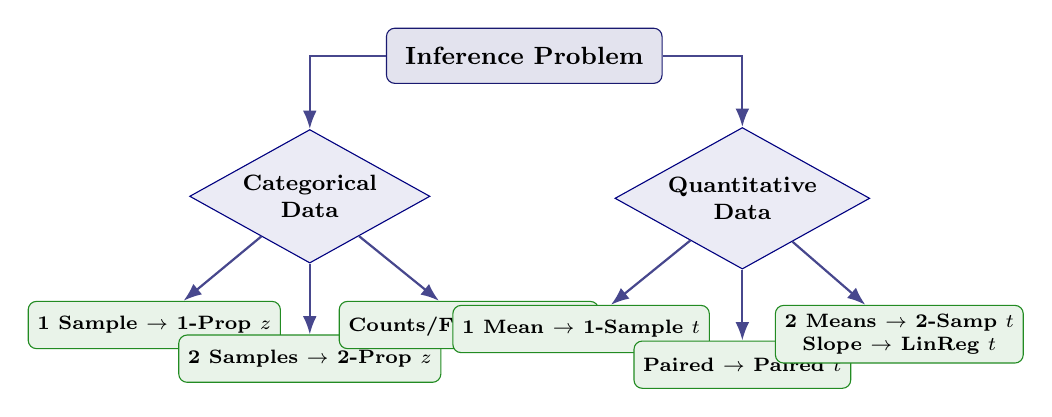
\begin{tikzpicture}[
  node distance=1.1cm and 0.8cm,
  every node/.style={font=\footnotesize, align=center},
  boxroot/.style={rectangle, rounded corners=3pt, minimum width=3.5cm, minimum height=0.7cm, draw=MidnightBlue, fill=MidnightBlue!12, font=\bfseries\small},
  branch/.style={diamond, aspect=1.8, draw=NavyBlue, fill=NavyBlue!8, font=\bfseries\footnotesize, inner sep=2pt},
  leaf/.style={rectangle, rounded corners=3pt, minimum width=2.6cm, minimum height=0.6cm, draw=ForestGreen, fill=ForestGreen!10, font=\bfseries\scriptsize},
  edge/.style={draw=MidnightBlue!80, -Latex, thick}
]
  \node[boxroot] (root) {Inference Problem};
  \node[branch, below left=1.0cm and 0.2cm of root] (cat) {Categorical\\Data};
  \node[branch, below right=1.0cm and 0.2cm of root] (quant) {Quantitative\\Data};
  
  \node[leaf, below left=0.9cm and -0.4cm of cat] (c1) {1 Sample $\rightarrow$ 1-Prop $z$};
  \node[leaf, below=0.9cm of cat] (c2) {2 Samples $\rightarrow$ 2-Prop $z$};
  \node[leaf, below right=0.9cm and -0.4cm of cat] (c3) {Counts/Fit $\rightarrow$ $\chi^2$ Test};

  \node[leaf, below left=0.9cm and -0.4cm of quant] (q1) {1 Mean $\rightarrow$ 1-Sample $t$};
  \node[leaf, below=0.9cm of quant] (q2) {Paired $\rightarrow$ Paired $t$};
  \node[leaf, below right=0.9cm and -0.4cm of quant] (q3) {2 Means $\rightarrow$ 2-Samp $t$\\Slope $\rightarrow$ LinReg $t$};

  \draw[edge] (root) -| (cat);
  \draw[edge] (root) -| (quant);
  \draw[edge] (cat) -- (c1);
  \draw[edge] (cat) -- (c2);
  \draw[edge] (cat) -- (c3);
  \draw[edge] (quant) -- (q1);
  \draw[edge] (quant) -- (q2);
  \draw[edge] (quant) -- (q3);
\end{tikzpicture}%
}
\end{center}

\vspace{0.2in}
\section{Inference Procedures Lookup Matrix}

\begin{table}[H]
\centering
\scriptsize
\begin{tabularx}{\linewidth}{@{}p{0.18\linewidth} p{0.17\linewidth} p{0.16\linewidth} X p{0.22\linewidth}@{}}
\toprule
\textbf{Data Type} & \textbf{Groups} & \textbf{Goal} & \textbf{Procedure Name} & \textbf{Calculator Command} \\
\midrule
Categorical & 1 Sample & Estimate $p$ & \textbf{1-Prop $z$-Interval} & \texttt{1-PropZInt} \\
Categorical & 1 Sample & Test $p$ & \textbf{1-Prop $z$-Test} & \texttt{1-PropZTest} \\
Categorical & 2 Samples & Estimate $p_1 - p_2$ & \textbf{2-Prop $z$-Interval} & \texttt{2-PropZInt} \\
Categorical & 2 Samples & Test $p_1 = p_2$ & \textbf{2-Prop $z$-Test (Pooled)} & \texttt{2-PropZTest} \\
Categorical & 1 Sample (Fit) & Fit distribution & \textbf{$\chi^2$ GOF-Test} & \texttt{$\chi^2$ GOF-Test} \\
Categorical & 2+ Samples & Homogeneity & \textbf{$\chi^2$ Test of Homogeneity} & \texttt{$\chi^2$-Test} (Matrix) \\
Categorical & 1 Sample (2 Var) & Association & \textbf{$\chi^2$ Test of Independence} & \texttt{$\chi^2$-Test} (Matrix) \\
\midrule
Quantitative & 1 Sample & Estimate $\mu$ & \textbf{1-Sample $t$-Interval} & \texttt{TInterval} \\
Quantitative & 1 Sample & Test $\mu$ & \textbf{1-Sample $t$-Test} & \texttt{T-Test} \\
Quantitative & Matched Pairs & Difference $\mu_d$ & \textbf{Paired $t$-Test/Interval} & \texttt{T-Test} on $L_1 - L_2$ \\
Quantitative & 2 Indep Samples & Compare $\mu_1 - \mu_2$ & \textbf{2-Sample $t$-Test/Interval} & \texttt{2-SampTTest} \\
Quantitative & Linear Slope & Slope $\beta$ & \textbf{LinReg $t$-Test/Interval} & \texttt{LinRegTTest} \\
\bottomrule
\end{tabularx}
\end{table}

% UNIT 11
\chapter{Top 25 "Never Forget" AP Exam Traps}
\begin{enumerate}[label=\textbf{\arabic*.}]
    \item \textbf{NEVER say "Accept $H_0$":} Always write \emph{"Fail to reject $H_0$"}.
    \item \textbf{NEVER write "We prove $H_a$":} Write \emph{"We have convincing statistical evidence that [context]"}.
    \item \textbf{Hypotheses in parameters ($\mu, p, \beta$), NEVER statistics ($\bar{x}, \hat{p}, b$).}
    \item \textbf{Define parameters in context.}
    \item \textbf{Use comparative words when comparing distributions (greater, lesser).}
    \item \textbf{Include units on ALL quantitative statistics and interpretations.}
    \item \textbf{Don't forget the hat ($\hat{y}$) on regression equations.}
    \item \textbf{Correlation ($r$) measures LINEAR strength only.}
    \item \textbf{Association is NOT Causation.}
    \item \textbf{Blocking is for experiments; Stratification is for sampling.}
    \item \textbf{Mutually exclusive events are NEVER independent.}
    \item \textbf{Always ADD variances, NEVER add standard deviations.}
    \item \textbf{CLT applies to sampling distribution of $\bar{x}$ ($n \ge 30$), not individual data.}
    \item \textbf{Use $p_0$ for 1-Prop $Z$-Test Large Counts ($np_0 \ge 10, n(1-p_0) \ge 10$).}
    \item \textbf{Use $\hat{p}$ for 1-Prop $Z$-Interval Large Counts ($n\hat{p} \ge 10, n(1-\hat{p}) \ge 10$).}
    \item \textbf{Chi-square conditions require EXPECTED counts $\ge 5$, not observed counts.}
    \item \textbf{Chi-square df:} $\text{df} = (\text{rows}-1)(\text{cols}-1)$.
    \item \textbf{Never pool standard deviations for 2-sample $t$-tests (\texttt{Pooled = NO}).}
    \item \textbf{Confidence Interval (plausible values) vs Confidence Level (long-run capture rate).}
    \item \textbf{A high $r^2$ does NOT prove linearity (always check residual plot).}
    \item \textbf{Voluntary response produces extreme bias.}
    \item \textbf{State the conclusion in terms of $H_a$.}
    \item \textbf{State the significance level ($\alpha$).}
    \item \textbf{Calculator Speak is NOT enough on FRQs (write formulas, df, $p$-value).}
    \item \textbf{Context, Context, Context: Include problem context in every sentence!}
\end{enumerate}

% UNIT 12
\chapter{Standard Interpretation Sentence Templates}
\begin{templatebox}[Template 1: Confidence Interval for a Parameter]
\emph{"We are [C\%] confident that the interval from [Lower Bound] to [Upper Bound] captures the true [proportion / mean] of [context with units]."}
\end{templatebox}

\begin{templatebox}[Template 2: Confidence Level ($C\%$)]
\emph{"If we take many random samples of size $n$ and construct [C\%] confidence intervals, about [C\%] of the intervals will capture the true [parameter in context]."}
\end{templatebox}

\begin{templatebox}[Template 3: $p$-Value in Context]
\emph{"Assuming that [null hypothesis $H_0$ in context] is true, there is a [p-value] probability of obtaining a sample statistic as extreme as or more extreme than observed, purely by random chance."}
\end{templatebox}

\begin{templatebox}[Template 4: Test Conclusion (Reject $H_0$)]
\emph{"Because $p$-value ($[p]$) $< \alpha$ ($[0.05]$), we reject $H_0$. There is convincing statistical evidence that [state $H_a$ in context]."}
\end{templatebox}

\begin{templatebox}[Template 5: Test Conclusion (Fail to Reject $H_0$)]
\emph{"Because $p$-value ($[p]$) $> \alpha$ ($[0.05]$), we fail to reject $H_0$. There is NOT convincing statistical evidence that [state $H_a$ in context]."}
\end{templatebox}

\end{document}

